\documentclass[presentation]{beamer}
\setbeamertemplate{navigation symbols}{}
\usepackage{graphicx}
\usepackage{caption}
\usepackage{xcolor}
\usetheme{Madrid}
\setbeamerfont{title}{size=\Large}
\setbeamerfont{normal text}{size=\small}

\title{Heuristic Performance Analysis}
\author{Afzal Hossan - 2005021}
\date{}

\begin{document}

\frame{\titlepage}

\section{Visualizations Comparing Heuristic Performances}

\begin{frame}{Average Optimized Distance by Heuristic Combination}
\begin{itemize}
    \item This bar graph compares the average optimized distances achieved by each heuristic combination.
    \item It helps identify which heuristics produce shorter routes on average.
\end{itemize}
\begin{center}
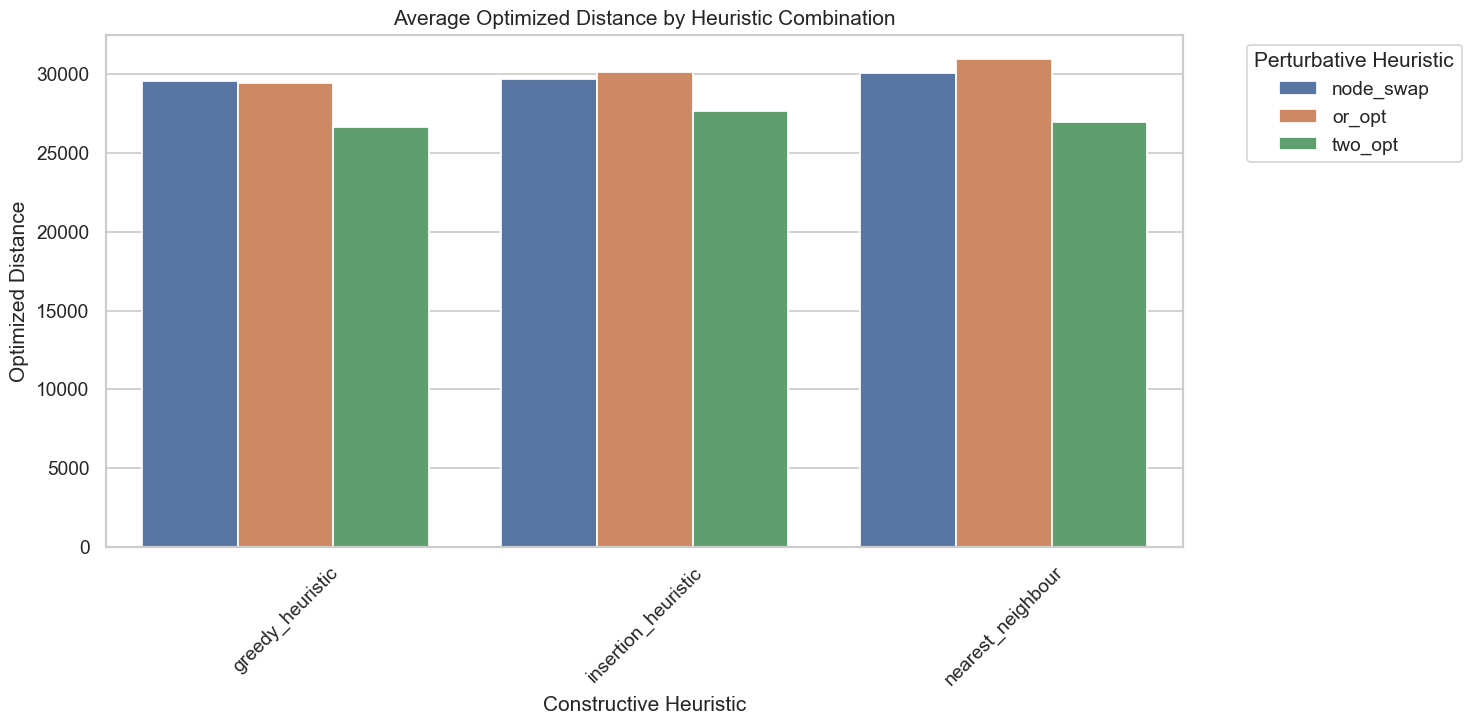
\includegraphics[width=0.75\textwidth]{average_distance_chart.png}\\
\end{center}
\textbf{Comment:} The greedy heuristic performs better than other constructive algorithms. The combination of the two\_opt heuristic with the greedy heuristic as a perturbative algorithm outperforms other combinations.
\end{frame}

\begin{frame}{Distance Improvement (\%) by Heuristic Combination}
\begin{itemize}
    \item This bar chart shows the average distance improvement for each combination of constructive and perturbative heuristics.
    \item Highlights which combinations lead to the largest improvements in route distance.
\end{itemize}
\begin{center}
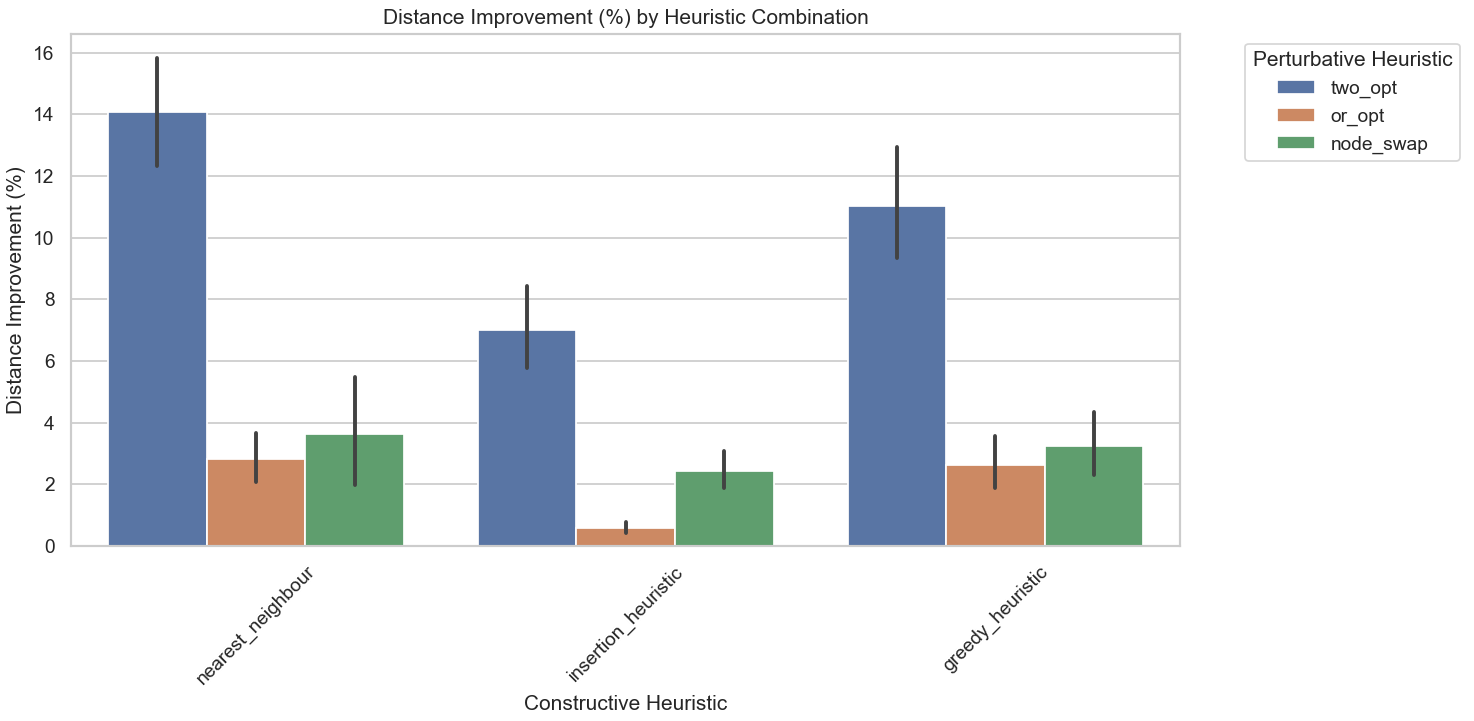
\includegraphics[width=0.75\textwidth]{distance_improvement_chart.png}\\
\end{center}
\textbf{Comment:} The two\_opt heuristic consistently performs the best, while the or\_opt heuristic performs the worst.
\end{frame}

\begin{frame}{Box Whisker Plot}
\begin{itemize}
    \item Box plots show the distribution of distance improvements by heuristic, which can reveal consistency. Some heuristics might achieve good improvements on average but with high variability.
\end{itemize}
\begin{center}
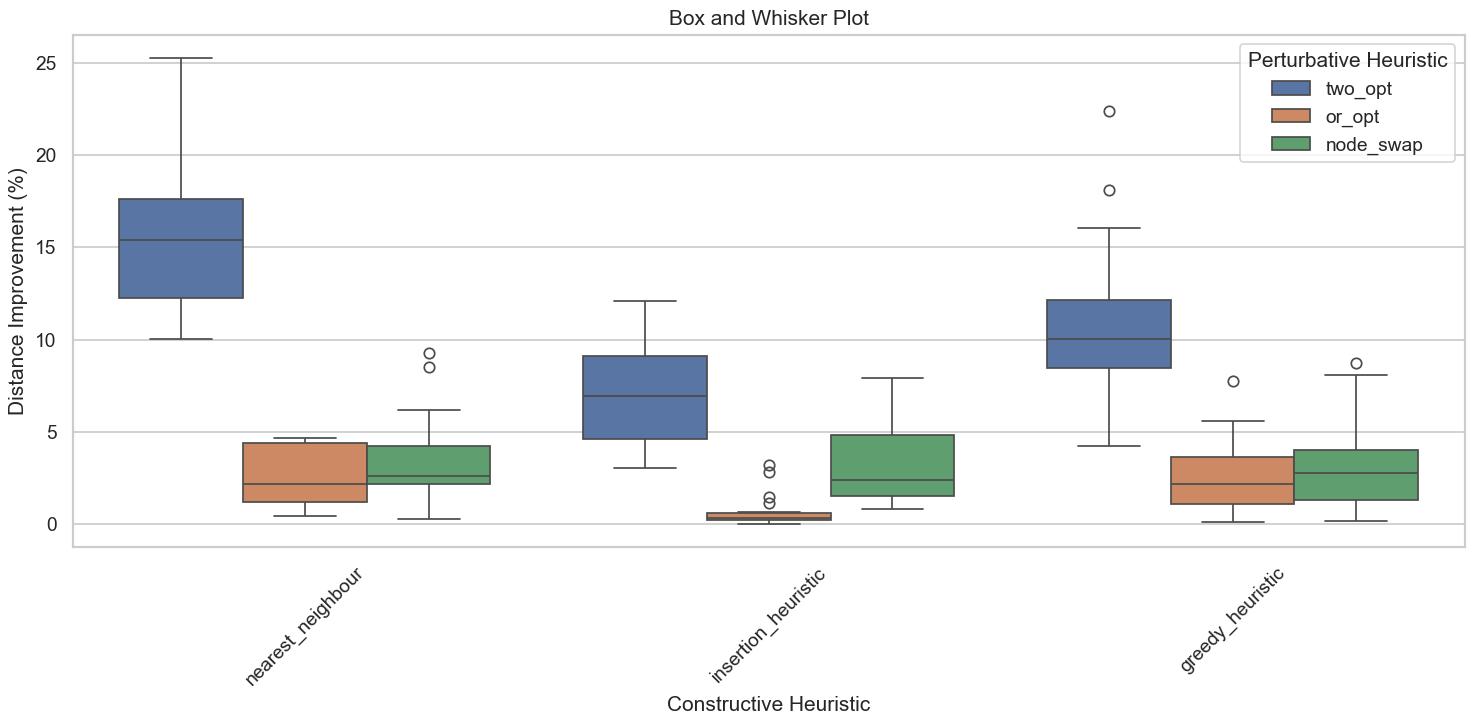
\includegraphics[width=0.8\textwidth]{Box_Whisker_Plot.png}\\
\end{center}
\textbf{Comment:} The Box Whisker Plot indicates that the combination of two\_opt and the greedy heuristic performs the best on average.
\end{frame}

\begin{frame}{Time Efficiency by Heuristic Combination}
\begin{itemize}
    \item This scatter plot shows the time required per unit of distance improvement.
    \item Combinations closer to the bottom indicate more time-efficient heuristics for each percentage of improvement in distance.
\end{itemize}
\begin{center}
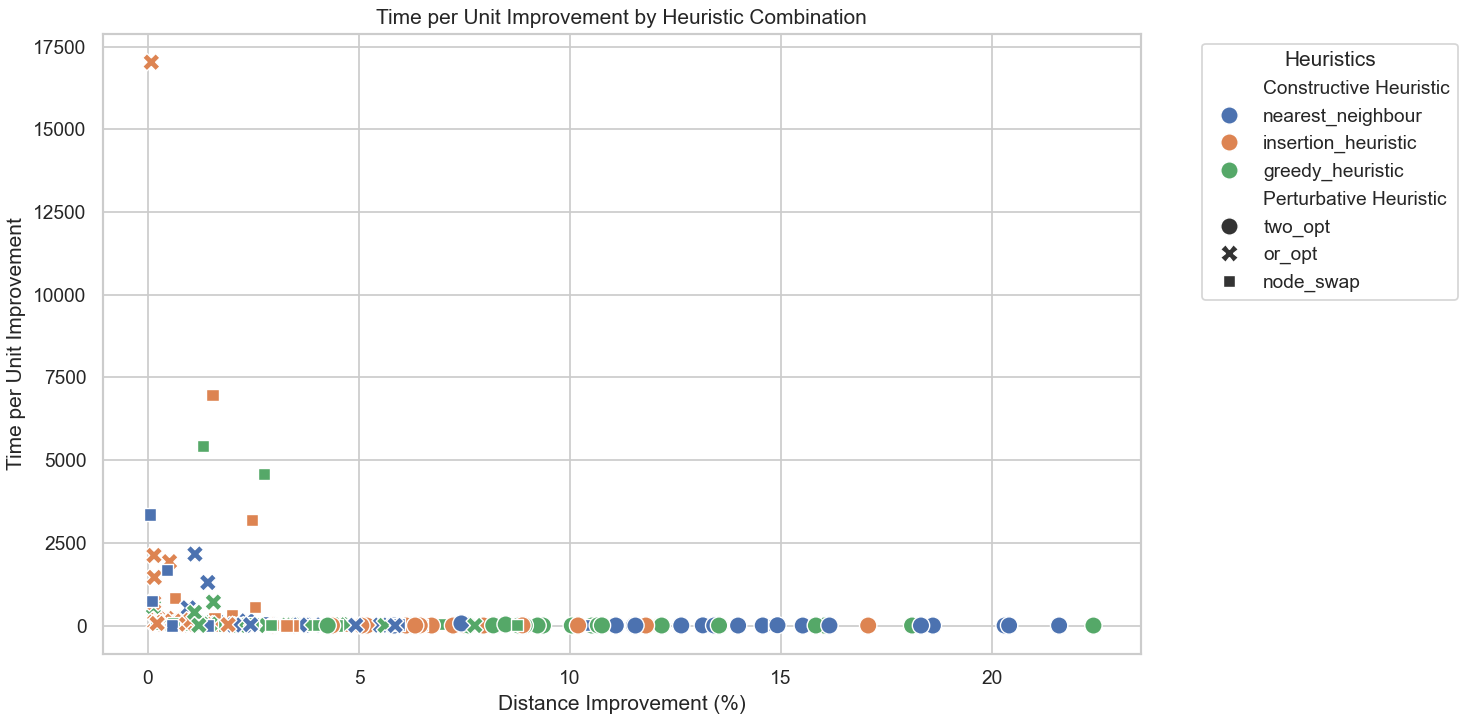
\includegraphics[width=0.75\textwidth]{time_efficiency_plot.png}\\
\end{center}
\textbf{Comment:} The two\_opt heuristic requires the least time per unit of distance improvement, while the or\_opt heuristic requires the most.
\end{frame}

\begin{frame}{Heuristic Efficiency Heat map}
\begin{itemize}
    \item This heat map shows the average optimized distance and/or time per unit of improvement for each combination.
    \item It provides an overview of which combinations yield the best results.
\end{itemize}
\begin{center}
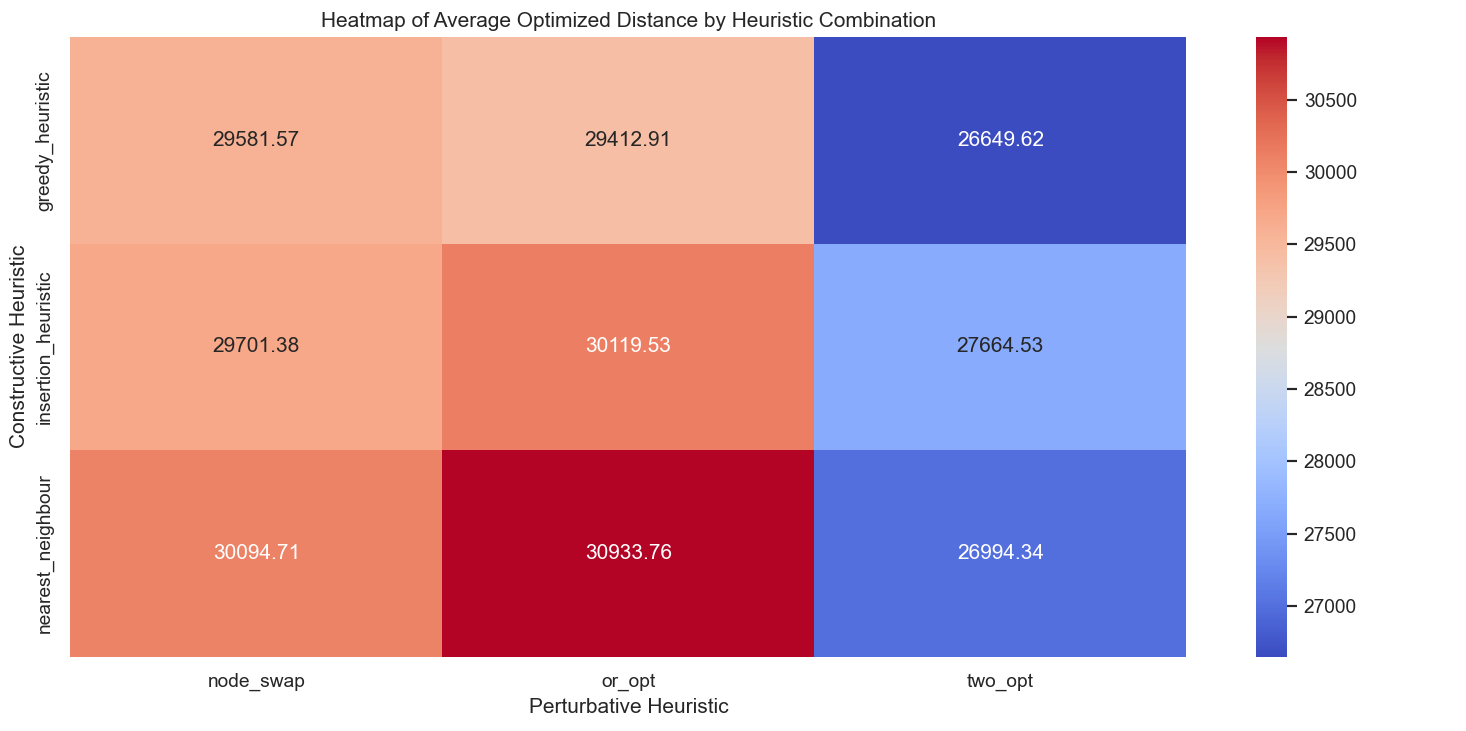
\includegraphics[width=0.7\textwidth]{heatmap.png}\\
\end{center}
\textbf{Comment:} The heat map indicates that the combination of two\_opt and the greedy heuristic performs the best on average. Conversely, the combination of or\_opt and the nearest-neighbor heuristic performs the worst.
\end{frame}

\end{document}
